%% Template for a preprint Letter or Article for submission
%% to the journal Nature.
%% Written by Peter Czoschke, 26 February 2004
%%

\documentclass[pdftex]{nature}
\usepackage{amsmath}
\usepackage{graphicx}
\usepackage{times}
\usepackage{lineno} 
\usepackage{rotating} 
\usepackage{color}
\usepackage{supertabular}

%% make sure you have the nature.cls and naturemag.bst files where
%% LaTeX can find them

\def\sa#1#2{\sout{#1} \textcolor{red}{#2}} 
\def\sac#1{\textcolor{red}{[#1]}}

\bibliographystyle{naturemag}

\title{The ghost of nestedness in ecological networks}
%% Notice placement of commas and superscripts and use of &
%% in the author list

\author{Phillip P.A. Staniczenko$^{1}$, Jason C. Kopp$^{1}$ \& Stefano
  Allesina$^{1,2}$}

\begin{document}
\linenumbers
\maketitle

\begin{affiliations}
{\small
 \item {Dept. Ecology \& Evolution, University of Chicago. 1101
   E. 57th Chicago, IL 60637 USA.}
 \item {Computation Institute, University of Chicago.}
}
\end{affiliations}

\begin{abstract}
Ecologists are fascinated by the prevalence of nestedness in
biogeographic and community data, where it is thought to promote
biodiversity in mutualistic systems.  Traditionally, nestedness has
been treated in a binary sense: species and their interactions are
either present or absent, neglecting information on abundances and
interaction frequencies.  Extending nestedness to quantitative data
facilitates the study of species preferences, and we propose a new
detection method that follows from a basic property of bipartite
networks: large dominant eigenvalues are associated with highly nested
configurations.  We show that complex ecological networks are binary
nested, but quantitative preferences are non-nested, indicating
limited consumer overlap of favoured resources.  The spectral graph
approach provides a formal link to local dynamical stability analysis,
where we demonstrate that nested mutualistic structures are minimally
stable.  We conclude that, within the binary constraint of interaction
plausibility, species preferences are partitioned to avoid
competition, thereby benefiting system-wide resource allocation.
\end{abstract}

Nestedness has been studied in a wide range of ecological systems.
The concept was first proposed in the early Twentieth Century but only
became popular among ecologists with its application to the
biogeographic pattern of species occurrence in islands and other
fragmented landscapes\cite{Patterson_Atmar, Patterson_only}.  More
recently, nestedness in species interaction networks has received
significant
attention\cite{Discrepancy,BascompteNestedness,rezende2007,almeida2008consistent,saavedra2011},
where it has been suggested that a nested pattern of interactions
leads to greater biodiversity in mutualistic systems such as
plant-pollinator networks\cite{Bastolla2009,TFScience2010}.  In a
nested bipartite network or graph, interactions are organised such
that specialists (e.g., pollinators that visit few plants) interact
with subsets of the species with whom generalists (e.g., pollinators
that visit many plants) interact.  A nested structure corresponds to a
systematic arrangement of non-zero entries in the binary matrix used
to represent a network, and existing detection methods are based on
distinguishing the nested pattern from other possible arrangements of
matrix
elements\cite{Ulrich_Almeida-Neto_Gotelli_2009,gotelliulrich2012}.
However, these methods are often computationally expensive for large
matrices and are not applicable to quantitative networks (binary
metrics extended to work with quantitative data, such as
WNODF\cite{WNODF}, do not make full use of the available quantitative
information).

Quantitative networks contain the number or frequency of pairwise
interactions between species, and we show how empirical data can be
rescaled to permit investigation of feeding or visitation preferences
in addition to basic presence-absence structure.  If preferences are
quantitatively nested then the most generalist resources are preferred
by all consumers---most strongly by generalist consumers, closely
followed by specialist consumers---and specialist resources are
neglected.  We formally extend the definition of nestedness to include
quantitative networks and propose a new and robust detection method
based on the eigenvalue spectrum of a graph's adjacency matrix.  The
spectral properties of perfectly nested graphs were first discussed in
the mathematical literature, where they are known as Double Nested
Graphs (DNGs)\cite{andelic2011bounds} or chain
graphs\cite{bhattacharya2008first}, and we show that large dominant
eigenvalues are associated with highly nested structures (for both
binary and quantitative matrices).  A spectral method has the
advantage that the eigenvalues of a matrix can be computed extremely
quickly---even for large matrices---and results are invariant to
matrix permutation\cite{SpectralGraphTheory}.

Of 52 bipartite ecological networks from the literature, including
plant-pollinator, parasitoid-host, and seed dispersal types, 51 (98\%)
were binary nested, however, only 3 (6\%) had preference structures
that were quantitatively nested.  These results agree with our
analysis of the dynamical (local) stability of nested graphs, where we
demonstrate that perfectly nested configurations are minimally stable.
Within the restriction of interaction plausibility---whether an
interaction is forbidden or not, and identifiable with binary
structure\cite{ForbiddenLinks}---species preferences are partitioned
to avoid competition.  Thus, ecological systems are organised such
that niches are exploited and the efficient use of available resources
is promoted.
  
 \section*{Results}
 \vspace{-0.5cm}
 Before explicitly considering ecological systems and
 empirical data, we begin by formally defining nestedness for both
 binary and quantitative bipartite networks, and present a general
 detection method that follows naturally from the matrix properties of
 nested graphs.

A bipartite network or graph contains $S$ nodes (species) that can be
partitioned into two disjoint sets $A$ (animals in pollination
networks) and $P$ (plants) such that each of the $E$ undirected edges
(an animal-plant interaction) connects a node in the set $A$ with one
in the set $P$.  For the binary case, the adjacency matrix $\mathcal
A$ is a square matrix in which $\mathcal A_{ij}=1$ if $i$ and $j$ are
connected and is zero otherwise; for quantitative networks $\mathcal
A_{ij}$ can take positive non-zero values other than 1.  The set of
eigenvalues are an invariant property of a matrix (they do not change
if rows or columns are permuted).  Because $\mathcal A$ is a symmetric
matrix all of its eigenvalues are real, and because the graph is
bipartite the eigenvalues are distributed symmetrically about zero.
The largest eigenvalue of $\mathcal A$ is known as its spectral radius
$\rho(\mathcal A)$, and for binary matrices its value is bounded from
above by $\sqrt{|E|}$\cite{andelic2011bounds,SpectralGraphTheory}.

Since matrix $\mathcal A$ is symmetric and the graph bipartite, we
need draw only the $|P| \times |A|$ incidence matrix $\mathcal B$
(e.g., Figure 1).  Nestedness can be defined as a property of the
matrix $\mathcal B$.  If $\mathcal B$ is a perfectly nested binary
matrix then there exists a permutation of rows and columns such that
the set of edges in each row $i$ contains the edges in row $i+1$,
while the set of edges in each column $j$ contains those in column
$j+1$.  More formally, the rows and columns of $\mathcal B$ can be
sorted (with $\mathcal B_{1,j}>0$ $\forall j$ and $\mathcal B_{i,1}>0$
$\forall i$) such that $\mathcal B_{i,j} \leq \min \left(\mathcal
B_{i,j-1}, \mathcal B_{i-1,j} \right)$.

This definition of perfect nestedness extends to quantitative as well
as binary matrices.  Matrices $A$, $C$, $D$, $I$, $K$ and $N$ in
Figure 1 are perfectly nested, as is matrix $C$ in Figure 2, while the
others are not.

In the mathematical literature regarding DNGs, Bell \emph{et
  al.}\cite{bell2008graphs} provide a theorem that states: among all
the connected bipartite graphs with $|S|$ nodes and $|E|$ edges, the
one yielding the largest spectral radius $\rho(\mathcal A)$ is a
perfectly nested graph. It was subsequently proved that the same holds
if the number of nodes in each set $P$ and $A$ are
fixed\cite{ProvePAE}, rather than choosing among all possible sizes
such that $|P|+|A|=|S|$ as in the original theorem. We confirm
numerically that among all the bipartite graphs with $|P|$ plants,
$|A|$ animals and $|E|$ edges, the configuration leading to the
largest spectral radius is a perfectly nested graph, with all other
perfectly nested graphs have spectral radii close to this maximum
value (Figure 1).  This finding extends to quantitative matrices and
quantitative nestedness (Figure 2).  The right tail of the spectral
radius distribution contains either perfectly nested graphs---of which
there can be many configurations (SI)---or graphs that are very close
to being perfectly nested, while the left tail contains graphs that
are far from being perfectly nested.  The spectral radius therefore
represents a natural scale for nestedness, with larger $\rho(\mathcal
A)$ obtained for more nested matrices, and we have developed a set of
statistical tests to determine the significance of nestedness for
matrices that are not necessarily perfectly nested.

Remarkably, matrices that are significantly non-nested in their binary
form become significantly nested when a nested quantitative pattern is
overlaid.  This suggests that the quantitative structure of a network
is likely to dominate any underlying binary pattern (SI).

The eigenvector associated with the spectral radius measures the
contribution of each node in the graph to nestedness, which besides
being of interest in its own right\cite{GoogleFW}, provides a natural
way of ordering nodes that best illustrates matrix nestedness.  This
follows from the standard eigenvalue equation $\mathcal A \, \vec{x} =
\lambda \vec{x}$: Because any eigenvector $\vec{x}$ multiplied by the
original adjacency matrix $\mathcal A$ yields a vector parallel to the
original adjacency matrix, the spectral radius (dominant eigenvalue)
represents a scale factor $\lambda$ for the dominant eigenvector.
Conversely, if the spectral radius is understood to be a measure of
nestedness, then the entries of the dominant eigenvector (of size the
number of species) represent the weighting of each species with
respect to nestedness.

We now turn our attention to the specific case of ecological systems.
In general, interactions among species can be described by a set of
dynamical equations: $\frac{dx_i}{dt}=f(x_i) + g(x_i,\vec{x})$, where
$x_i$ is the density of a given species $i$, $f(x_i)$ describes the
effect of its density on population growth, and $g(x_i,\vec{x})$ is
the contribution to growth from interactions with other species in the
system\cite{rosenzweigmacarthur1963,hollanddeangelis2009,hollanddeangelis2010}.
We can divide the interaction term between two species,
$g(x_i,\vec{x})$, into two parts: the frequency of interactions
$\gamma_{i,j} x_i x_j$, and the effect of each interaction
$h(x_i,\vec{x})$, and so $g(x_i,\vec{x})=\sum_j \gamma_{i,j} x_i x_j
h(x_i,\vec{x})$.  Typically, $h(x_i,\vec{x})$ takes the form of a
functional response that captures the effect of an interaction between
$i$ and all of its partners $\vec{x}$ (e.g., Holling's Type
II\cite{HollingType21959}).  For each pair of species, $x_i x_j$ is a
mass action term, and $\gamma_{i,j}$ indicates the relative frequency
or probability of interaction compared to mass action.  Under the mass
action hypothesis the basic affinity between two species---the
expected magnitude of encounters---is directly proportional to the
product of their densities, and factors such as the spatial layout of
the environment, consumer search efficiency or handling time are not
accounted for. These additional factors are aggregated in
$\gamma_{i,j}$.  For each plausible ($\gamma_{i,j} \neq 0$)
interaction, $\gamma_{i,j}$ can be thought of as a preference
parameter: if $\gamma_{i,j}>1$ then the interaction is more likely to
occur than expected and is therefore favoured, $\gamma_{i,j}<1$
indicates that the interaction is less favorable, and $\gamma_{i,j}=1$
is exactly the expectation based on mass action.  When we record
ecological data such as the number of pollinator-plant visits---data
that can be organised in the form of a quantitative incidence matrix
$\mathcal B$---we implicitly record $\mathcal B_{i,j} = \gamma_{i,j}
x_i x_j$.  So in practice, empirical data must be adjusted for mass
action ($x_i x_j$) to isolate species preference $\gamma_{i,j}$.

We are particularly interested in whether the pattern of nestedness
observed in binary bipartite ecological
networks\cite{BascompteNestedness} is maintained in the quantitative
preference structure represented by the $\gamma-$matrix.  In a nested
quantitative network, generalist-generalist species interactions are
strongest, followed by generalist-specialist interactions, whereas
specialist-specialist interactions are much weaker (and may be absent
altogether).

Before applying the tests for nestedness to empirical data, we first
remove the effect of mass action in order to isolate species
preferences.  Since interaction data are rarely accompanied by
independent measures of species density, we use a method based on
solving overdetermined sets of equations\cite{pseudoinverse} to infer
effective species abundances from quantitative interaction networks.
These effective abundances should not be interpreted as
field-measurable equivalents, rather, they are best-fit abundances
under the mass action hypothesis. In some regards their use is more
appropriate than raw abundance data because they incorporate
confounding factors such as life-cycle turnover, partner co-occurrence
overlap, and unevenness in spatial distribution.

To obtain effective abundances recall that we can write empirical
count data $\mathcal B_{i,j} = \gamma_{i,j} x_i x_j$.  If no
interaction is recorded $\mathcal B_{i,j} = 0$ and we set the estimate
for species preference $\hat{\gamma}_{i,j} = 0$.  For the remaining
set of recorded counts with $\mathcal B_{i,j} > 0$, we take logarithms
$\log \mathcal B_{i,j} = \log \gamma_{i,j} + \log x_i + \log x_j$ and
perform a linear regression. However, rather than regressing ``y''
against ``x'' as is more commonly done, we do the opposite such that
we infer the log-transformed effective abundances $\hat{x}_i$ and
$\hat{x}_j$ from the log-transformed (non-zero) counts (SI).  The
preference $\gamma$-term then represents errors or residuals, and
since $\log \gamma_{i,j}$'s are minimised during regression the
estimated $\hat{\gamma}_{i,j}$'s are constrained to be as close to 1
as possible.  In this way, binary matrices can be seen as a special
case in which interaction magnitude is completely explained by mass
action.  And as required, preferences are scaled relative to mass
action---based on the inferred effective abundances---with
$\hat{\gamma}_{i,j} = \mathcal B_{i,j}/(\hat{x}_i \hat{x}_j)$.  This
quantitative $\hat{\gamma}-$matrix can be assessed for nested
patterns.


We tested 52 bipartite empirical networks for binary and quantitative
nestedness (Table 1).  For each network and test, we computed the
probability $p$ that a randomly constructed matrix $\mathcal A'$,
which preserves some of the properties of the empirical matrix
$\mathcal A$, is associated with spectral radius $\rho(\mathcal A')
\ge \rho(\mathcal A)$ (SI).  All but one of the networks were binary
nested ($p<0.05$), in agreement with earlier
studies\cite{BascompteNestedness}.  However, nestedness was not
observed in species preferences: for the vast majority of networks,
the quantitative structure of the $\hat{\gamma}-$matrix was
indistinguishable from random configurations, and in some cases,
anti-nestedness became apparent ($p>0.95$) (Table 1, Figure 3).  The
lack of nestedness in the dominant quantitative structure of empirical
networks is consistent with our mathematical treatment of the local
stability of nested structures.  Although capturing only one aspect of
ecological system dynamics, the mathematical tractability of local
stability analysis provides a good starting point for assessing the
dynamical consequences of network structure in its most simplistic
form\cite{StabilityCriteria}.

Local stability analysis is concerned with how a dynamical system
resting at equilibrium responds to perturbations.  If an equilibrium
point is stable, then the system returns to that point following small
perturbations.  For unstable equilibrium points, small perturbations
will move the system away from the original resting state.
Mathematically, the stability of an equilibrium point is completely
defined by the sign of the real parts of the eigenvalues of the
so-called community matrix
$M$\cite{levins1968evolution,may2001stability,StabilityCriteria}
(these eigenvalues are distinct from the adjacency matrix eigenvalues
we have been considering so far).  If all of the signs are negative
then the equilibrium point is stable.  Contemporary work has shown
that nested mutualistic networks are less likely to be stable than
their random counterparts\cite{StabilityCriteria}.  We now demonstrate
that a nested structure within $M$ minimises local stability.

A community matrix can be written as the sum of a matrix with zeros on
its diagonal, $M'$, and a corresponding diagonal matrix, $D$, i.e.,
$M=M'-D$.  For very large systems, the spectral radius of $M$ is
$\rho(M) \approx \rho(M') - \bar{D}$, where $\bar{D}$ is the average
value of the diagonal\cite{StabilityCriteria}.  Stability is therefore
achieved whenever $\rho(M') < \bar{D}$.  Analogous to arranging
coefficients in an adjacency or incidence matrix (as we did above),
among all possible ways of arranging the coefficients of $M'$ the
configuration yielding the largest spectral radius is perfect
nestedness (binary or quantitative).  (Note that the community matrix
is often considered non-symmetric, i.e., the effect of an animal on a
plant is often assumed to be different from that of the plant on the
animal.  However, the maximum spectral radius is obtained for
symmetric matrices.)  Hence, for a given diagonal and set of
coefficients, nestedness minimises local stability.

This is seemingly at odds with the prevailing view that nestedness
promotes the persistence of species in mutualistic
systems\cite{Bastolla2009,TFScience2010} (although recent work has
begun to question this proposition\cite{James2012}).  As an approach
to assessing system robustness, persistence encompasses local
stability analysis---in many models of mutualism, local stability
guarantees species persistence but locally unstable states may yet
display persistence.  Repeating precisely the analysis of Th\'ebault
\& Fontaine\cite{TFScience2010} we show that many dynamical models
inadvertently build-in trivial local stability and hence guarantee
persistence: the diagonal elements of the community matrix are always
large enough to compensate for the potential destabilising effect of
nestedness, thereby precluding nestedness---or, indeed, any other
configuration of interactions---from having a significant contribution
to local stability or persistence in such models (SI).  The claimed
positive relationship between nestedness and persistence actually
reflects a trivial positive relationship between connectance and
persistence in obligate mutualistic systems; Trivial because species
without partners immediately go extinct (a feature not considered by
Th\'ebault \& Fontaine\cite{TFScience2010}), and species with initial
densities close to zero will quickly go extinct unless they have
sufficient (binary) mutualistic partners to ``pull'' them to larger
densities, after which, they are guaranteed to
persist\cite{AllesinaComment}.

\section*{Discussion}
\vspace{-0.5cm}
Traditionally, nestedness has been associated with the
plausibility of interaction: if the length of a pollinator's proboscis
is sufficient to obtain nectar from plants with deep corolla tubes,
then it can also obtain nectar from species with shallower tubes,
otherwise its visitation partners are restricted---for a community
with many pollinator species, each with a different proboscis length,
a nested binary interaction pattern emerges.  Quantitative data allow
us to investigate whether pollinators interact with particular plants
more or less frequently than would be expected through random
encounter, and whether they do so in any systematic fashion.  With a
nested preference structure, almost all consumers disproportionately
interact with a common subset of the most generalist resources, while
ignoring more specialist resources.

While we found empirical networks to be binary nested, after adjusting
for uneven species abundances according to mass action, their
quantitative preference structures were distinctly non-nested.  The
need to account for abundances has been highlighted using synthetic
networks, where heterogeneous abundance distributions combined with
random species associations was sufficient to produce significantly
nested binary patterns, leading to the conclusion that complex
trait-based models were not necessary to explain
nestedness\cite{Bluthgen2008}.  Our results extend this argument to
quantitative networks: The vast majority of empirical networks
analysed had quantitative preference structures indistinguishable from
random graphs, meaning that no systematic process is required to
promote or constrain observed levels of nestedness.

The lack of quantitative nestedness also finds support from
mathematical analysis, where we showed that nested configurations of
mutualistic interactions are minimally stable from the perspective of
local stability analysis.  How other types of interaction---such as
antagonistic or facilitative pairings\cite{Bastolla2009}---formally
combine with mutualism to determine the overall stability and
persistence of a network requires further work.  At the community
level, compared to quantitatively nested preference structures,
non-nested structures suggest that species preferences are partitioned
to avoid competition.  Species rarely forgo abundant and accessible
resources, rather, less abundant resources are disproportionately
favoured by different sets of consumers---niches naturally arise.  It
would be instructive to see whether this kind of niche partitioning is
also apparent at the level of individuals within a single species
population\cite{Tinker2012}.

Much like the constituent elements of our sun can be inferred by
studying the solar spectrum of light, we used a spectral
approach---spectrum derived from the Latin for ghost---to detect
nestedness in complex ecological networks.  And like a ghost,
nestedness, which was strongly apparent in binary structures (although
the ecological significance of this observation is
debatable\cite{Bluthgen2008}), disappeared when quantitative
preference structures were analysed.  As the size of ecological data
grows, the advantages of a spectral approach will become more
pronounced; here we considered only the dominant eigenvalue of a
network's adjacency matrix, the relationship between other spectral
properties and ecological phenomena warrants further investigation.
Nestedness may not be the preeminent structure once thought, but
spectral analysis may yet offer clues as to what structural features
influence the function of large complex ecological networks.

\section*{References}
\vspace{-0.5cm}
\bibliography{BIBEigenNestshortJ}

\vspace{-0.6cm}
\begin{addendum}
 \item We thank A. Ekl\"of, J. Landau, F. Marquitti, C. Meli\'an,
   M. Pires and S. Tang for discussion.  Research supported by NSF EF
   \# 0827493 (S.A.) and NSF SMA \# 1042164 (P.P.A.S.).
   
\vspace{-0.25cm}
 \item[Competing Interests] The authors declare that they have no
   competing financial interests.
\vspace{-0.25cm}
\item[Contributions] P.P.A.S. and S.A. designed the analysis and
  performed the mathematical derivation.  S.A. wrote the
  code. J.C.K. obtained data and performed simulations. All authors
  wrote the manuscript.
\vspace{-0.25cm}
 \item[Correspondence] Correspondence should be addressed to
   P.P.A.S. (pstaniczenko@uchicago.edu).
\end{addendum}

\section*{Figure Captions}
\vspace{-0.5cm}
\noindent {\bf Figure 1.  Binary nestedness and eigenvalues.}
Spectral radius ($\rho$, largest eigenvalue) distribution for all
connected graphs with $|P|=6$, $|A|=4$ and $|E|=17$. There are 346,104
possible incidence matrices with this parameter combination, and of
these, 339,192 are connected (shown in figure).  Among the connected
graphs, 7,560 are perfectly nested (coloured orange), and have higher
spectral radii than most other matrices (all perfectly nested matrices
are contained in the top 4.59\% of the distribution).  The maximum
spectral radius is found for matrix $N$, and all matrices with
spectral radius greater than that of matrix $A$ are either perfectly
nested or very close to being perfectly nested (bottom series):
matrices $B$, $E$, $F$, $G$, $H$, $J$, $L$ and $M$ would become
perfectly nested if we were to move just one edge.  Matrices with the
lowest spectral radii depart most severely from perfect nestedness
(top series).

\noindent {\bf Figure 2.  Quantitative nestedness and eigenvalues.}
Spectral radius ($\rho$, largest eigenvalue) distribution for a
perfectly nested binary structure (matrix $A$ from Figure 1) with
randomised quantitative overlay.  A single set of $|E|=17$ coefficient
values are shuffled within the binary structure 10,000 times, and each
time the spectral radius is computed.  High spectral radius is
associated with a highly-nested quantitative configuration (e.g.,
matrix $C$, where darker colours indicate higher relative element
values), medium spectral radius with a non-specific quantitative
configuration (e.g., matrix $B$), and low spectral radius with an
anti-nested quantitative configuration (e.g., matrix $A$).  Thus, the
positive relationship between spectral radius and nestedness found for
binary matrices extends to quantitative matrices.

\noindent {\bf Figure 3.  Empirical nestedness.}  Three versions of a
seed-dispersal mutualistic network with $|P|=19$, $|A|=29$ and
$|E|=211$ (web 37 in SI).  In each incidence matrix darker colours
indicate higher relative element values, $p$-values are for 10,000
null model randomisations: a) binary network is nested with $p<0.001$;
b) empirical count quantitative interaction network is nested with
$p<0.05$; and c) quantitative preference structure,
$\hat{\gamma}$-matrix, is anti-nested, $p>0.95$.  Within the
restriction of interaction plausibility, i.e., not forbidden
interactions (matrix a) and after rescaling the raw data (matrix b)
according to mass action, species preferences are found to be
distributed in an anti-nested manner (matrix c).

\begin{table}
\caption{Nestedness of ecological networks using quantitative null
  model iv
\newline
	(maintain binary structure and shuffle non-zero coefficients)}
\centering
\begin{tabular*}{0.66\hsize}
{lrrrr}
Structure & nested & no pattern & anti-nested & Total\\
\hline
Binary & 51 (98\%) & 1 (2\%) & 0 (0\%) & 52\\
Preference & 3 (6\%) & 45 (86\%) & 4 (8\%) & 52\\
\hline
\end{tabular*}
\end{table}


\clearpage
\section*{Figures}
\noindent {\bf Figure 1.  Binary nestedness and eigenvalues.} 

 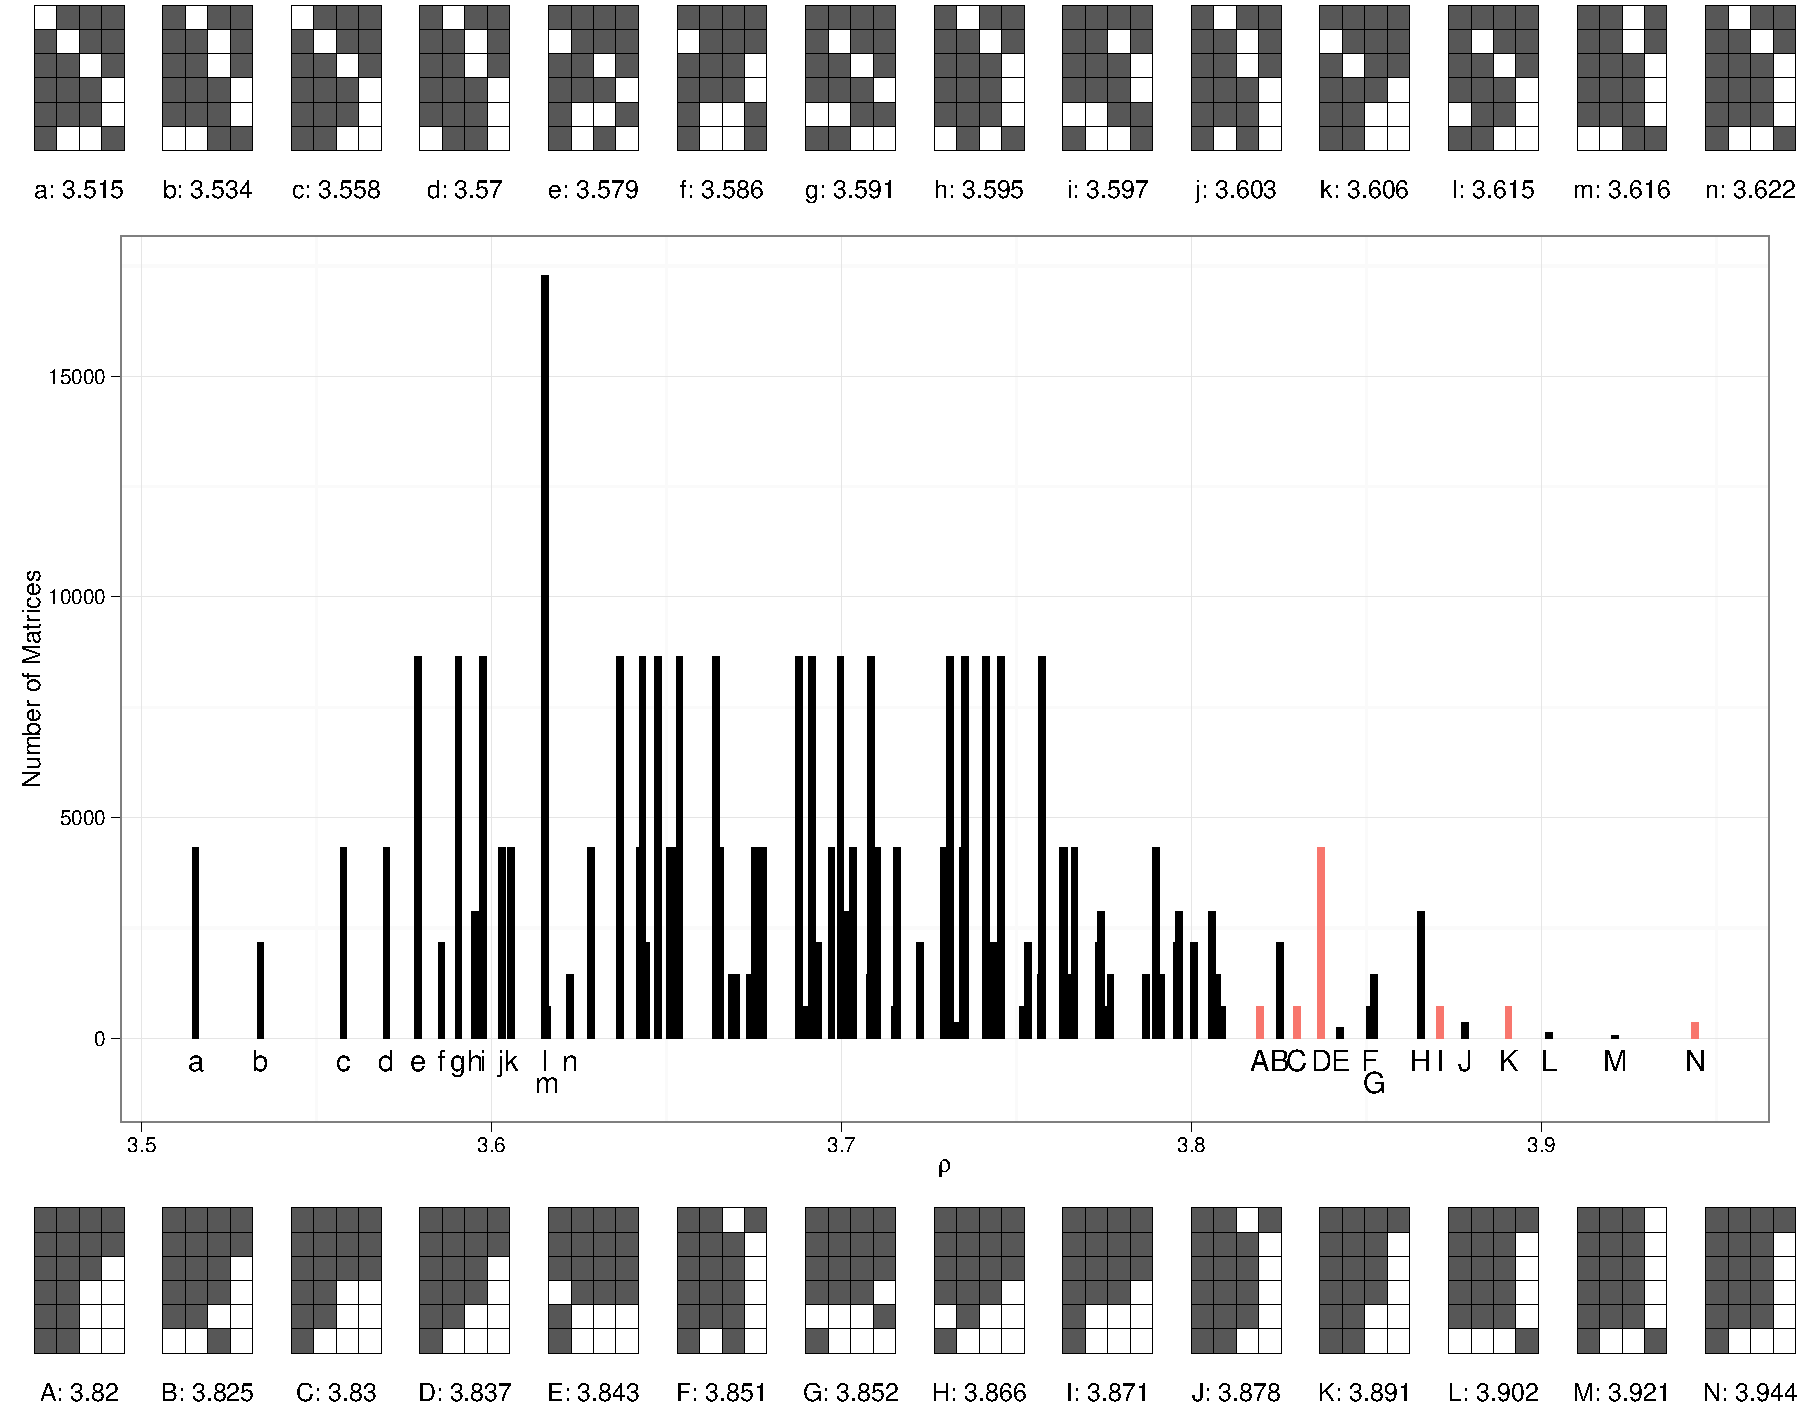
\includegraphics[width=0.9\textwidth]{Figures/Rho-17.pdf}

\newpage
\noindent {\bf Figure 2.  Quantitative nestedness and eigenvalues.} 

\begin{tabular}{l}
    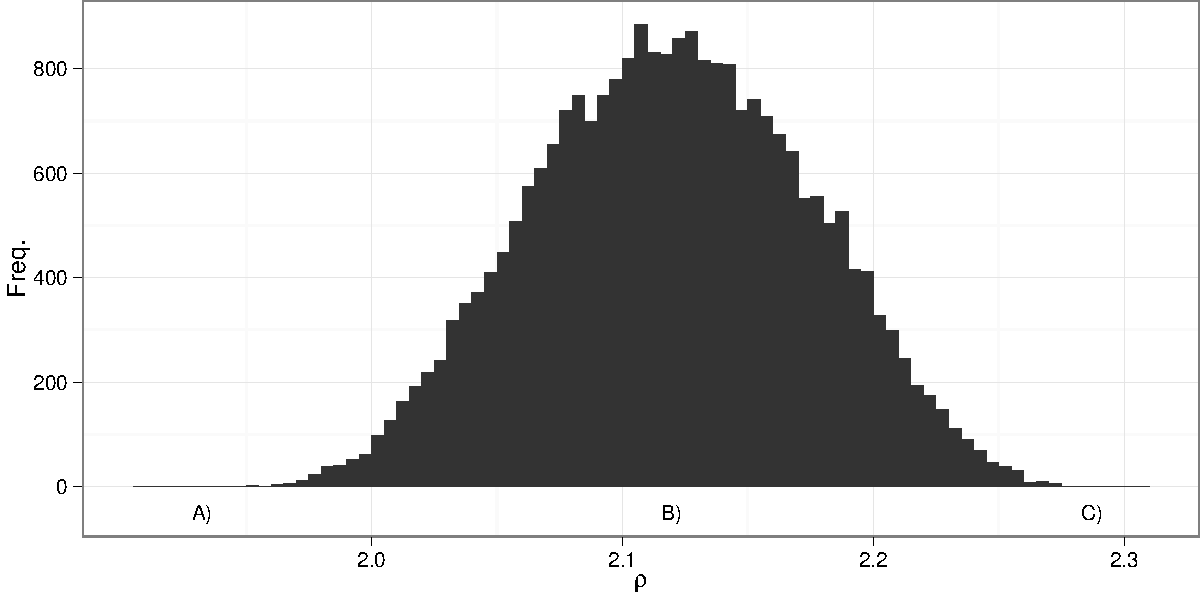
\includegraphics[width=0.8\textwidth]{Figures/FigQuant6-4-17-a.pdf}
  \end{tabular}
  \begin{tabular}{p{0.1\textwidth} }
    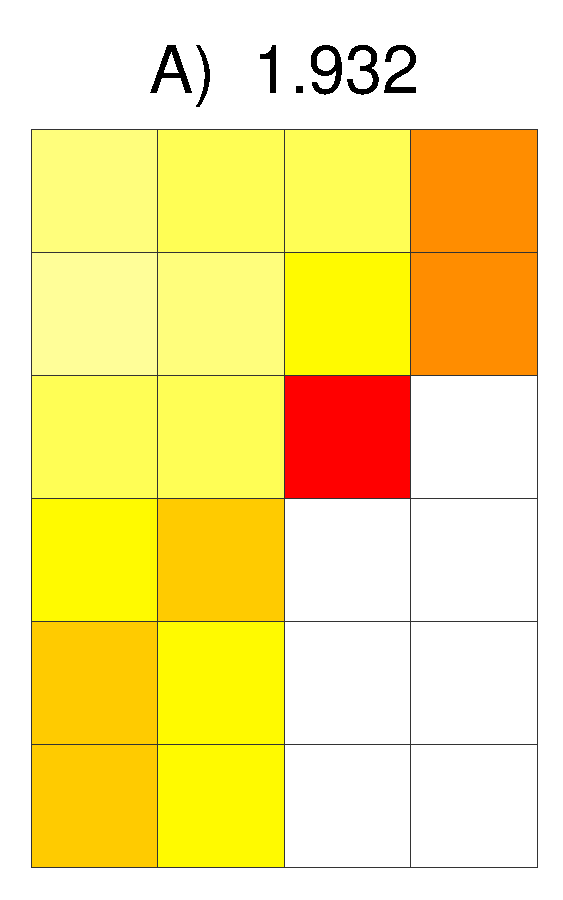
\includegraphics[width=0.08\textwidth]{Figures/Min-6-4-17.pdf}\\
    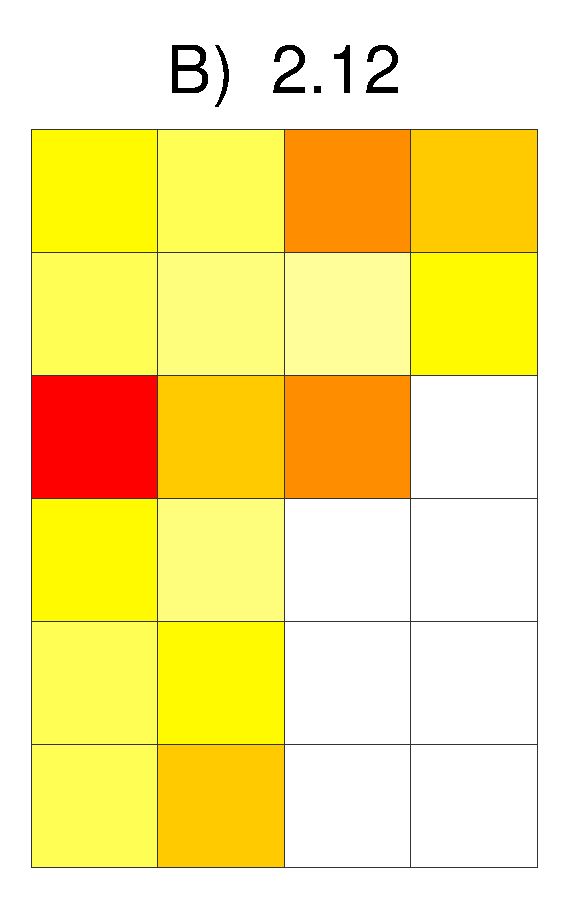
\includegraphics[width=0.08\textwidth]{Figures/Mean-6-4-17.pdf}\\
    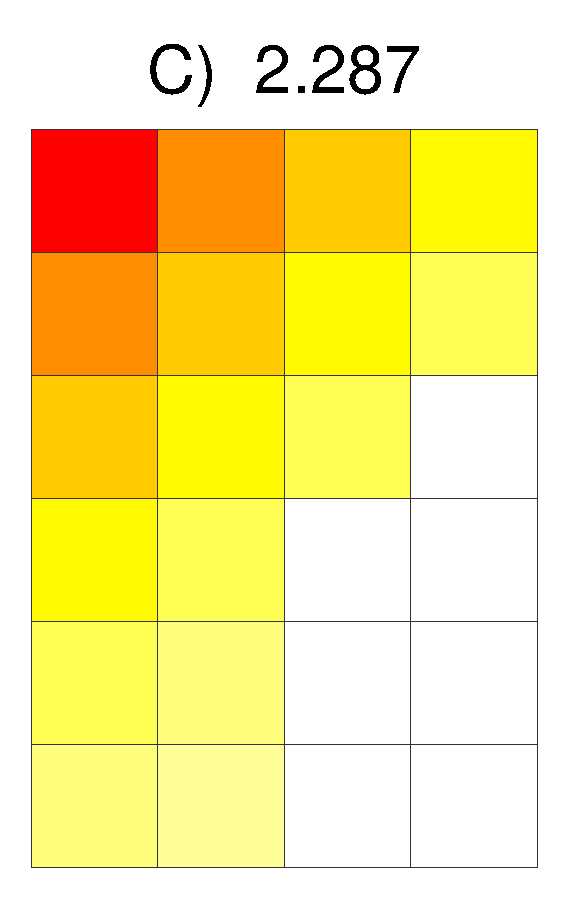
\includegraphics[width=0.08\textwidth]{Figures/Max-6-4-17.pdf}\\
  \end{tabular}

\vspace{3cm}
\noindent {\bf Figure 3.  Empirical nestedness.} 

  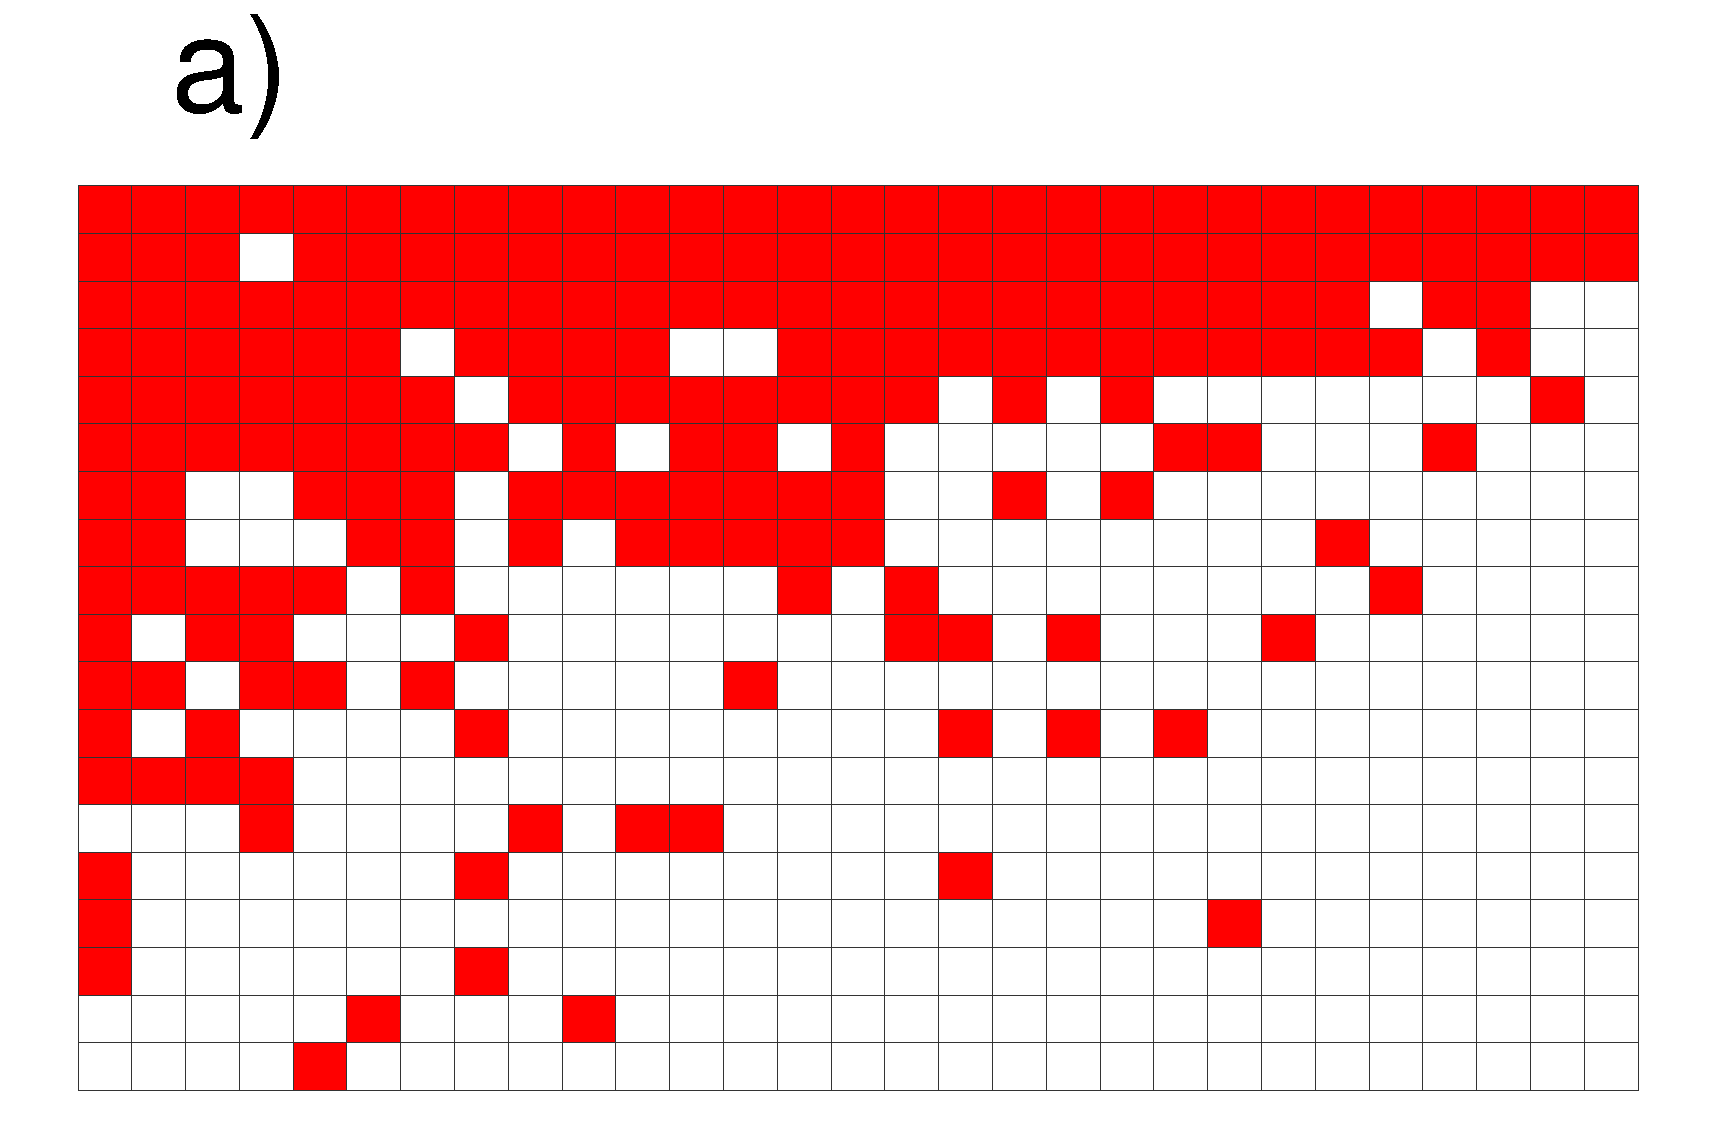
\includegraphics[width=0.32\linewidth]{Figures/p89_binary.pdf}
  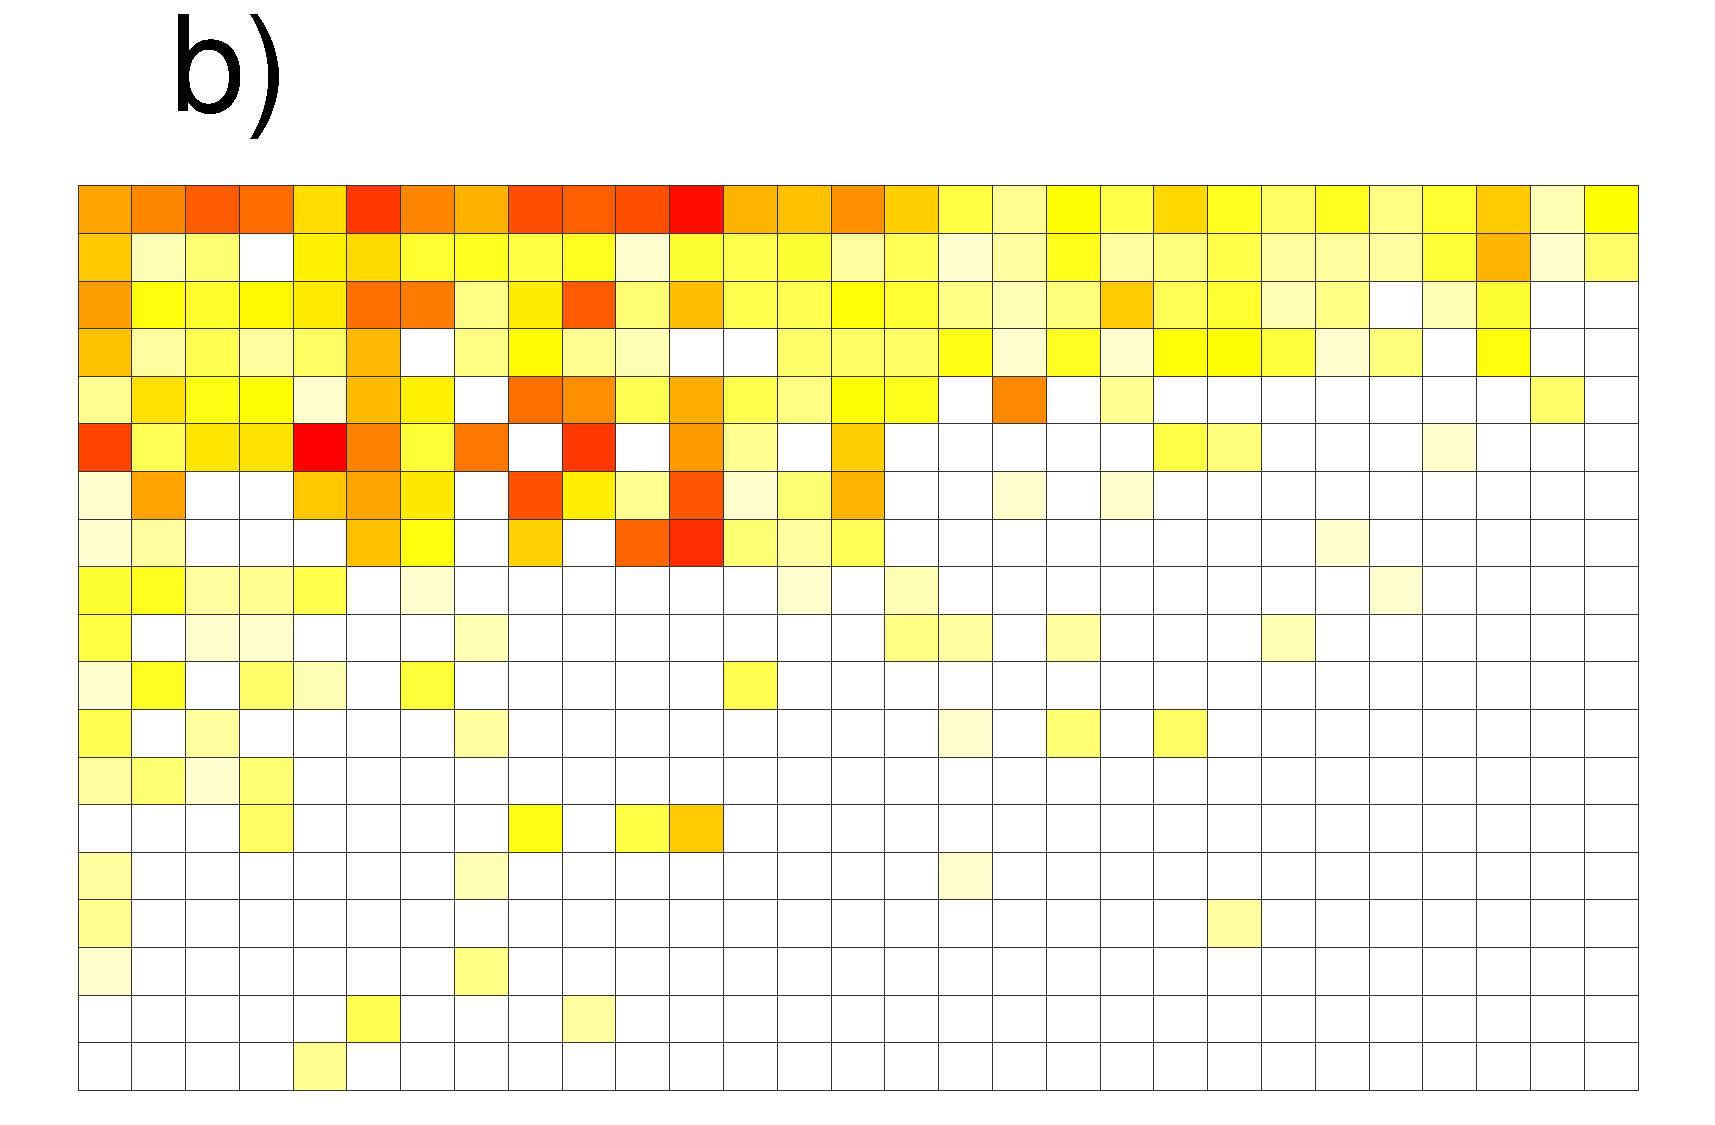
\includegraphics[width=0.32\linewidth]{Figures/p89_log_dual.pdf}
  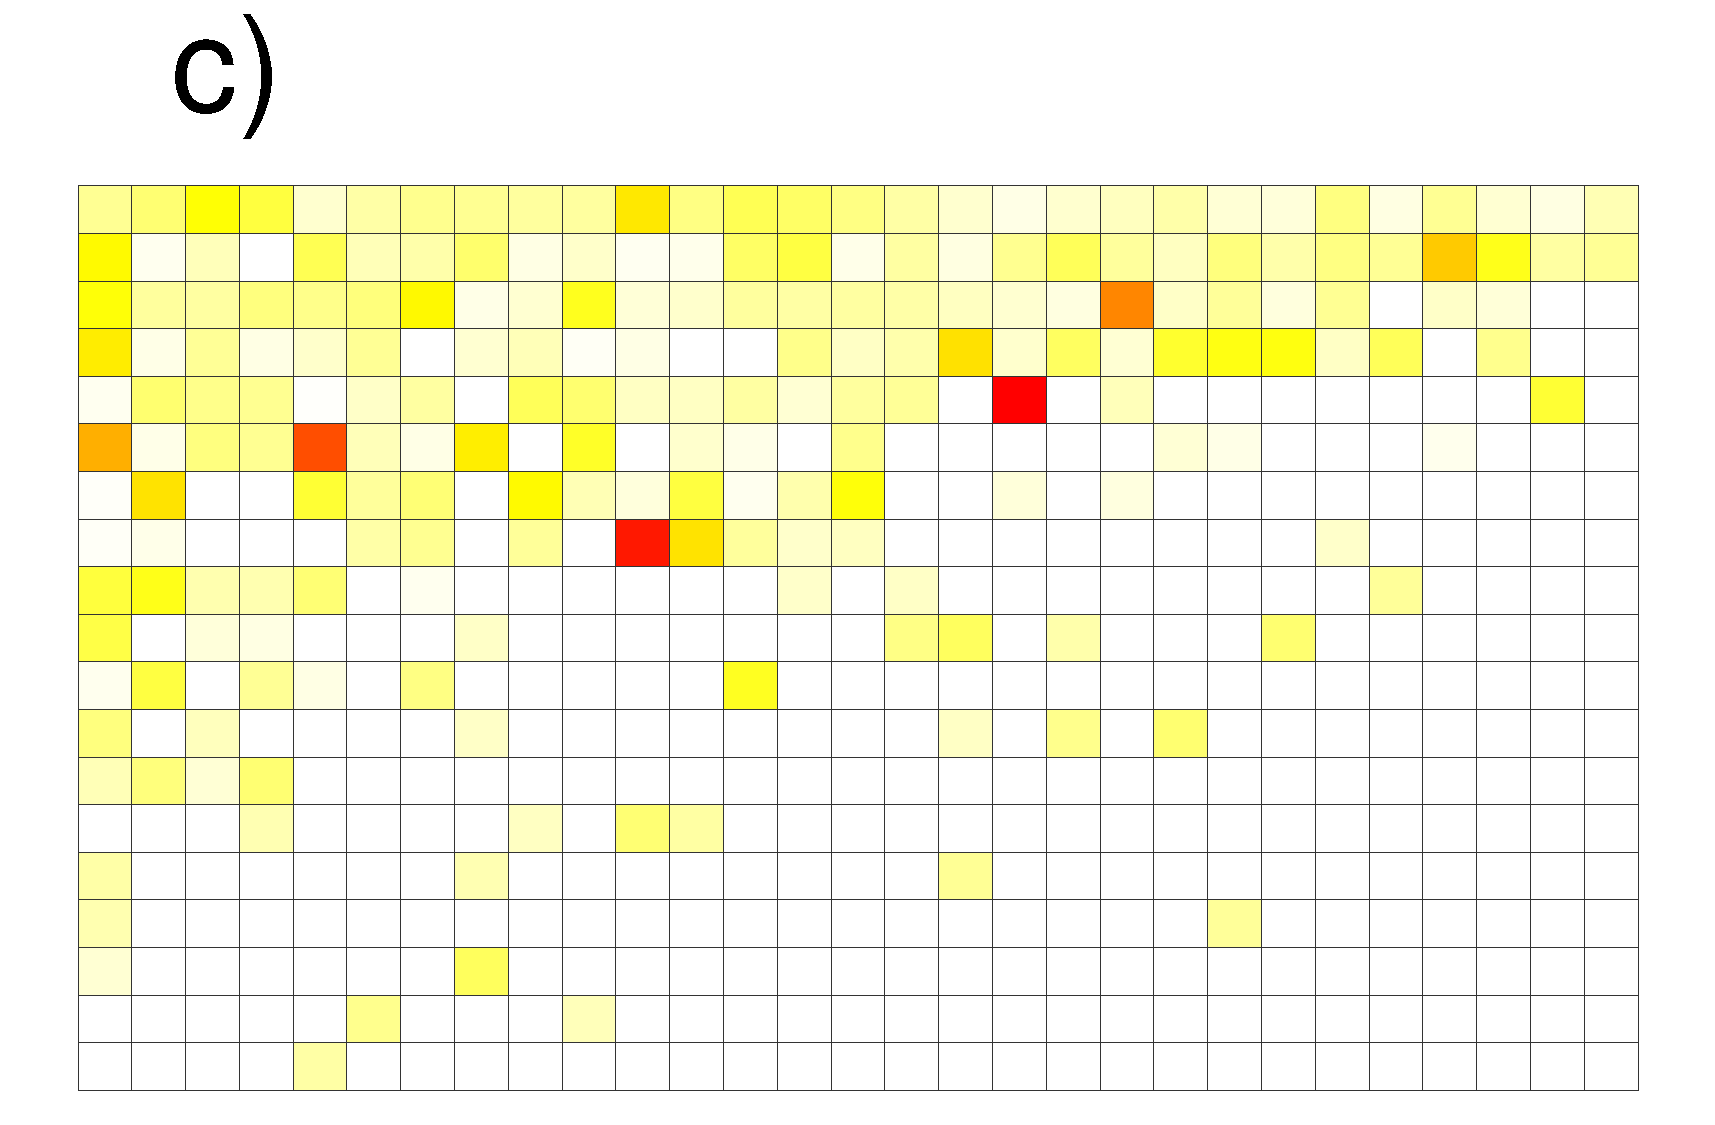
\includegraphics[width=0.32\linewidth]{Figures/p89_pref_log_dual.pdf}

\end{document}
